  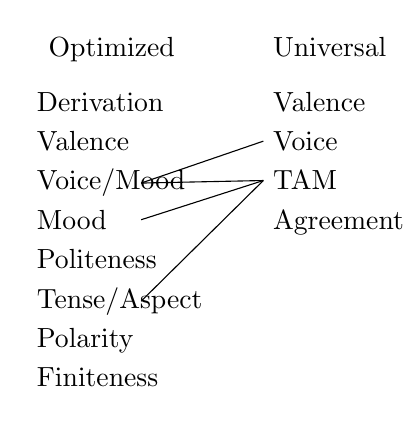
\begin{tikzpicture}[%
% common options for blocks:
block/.style = {draw, fill=blue!30, align=center, anchor=west,
            minimum height=0.65cm, inner sep=0},
% common options for the circles:
ball/.style = {circle, draw, align=center, anchor=north, inner sep=0}]
\node[rectangle,text width=1.2cm,anchor=base] (A0) at (4,-0.3) {Universal};
\node[rectangle,text width=0.9cm,anchor=base] (B0) at (1,-0.3) {Optimized};
\node[rectangle,text width=1.2cm,anchor=base] (A1) at (4,-1.0) {Valence};
\node[rectangle,text width=1.2cm,anchor=base] (A2) at (4,-1.5) {Voice};
\node[rectangle,text width=1.2cm,anchor=base] (A3) at (4,-2.0) {TAM};
\node[rectangle,text width=1.2cm,anchor=base] (A4) at (4,-2.5) {Agreement};
\node[rectangle,text width=1.2cm,anchor=base] (B1) at (1,-1.0) {Derivation};
\node[rectangle,text width=1.2cm,anchor=base] (B2) at (1,-1.5) {Valence};
\node[rectangle,text width=1.2cm,anchor=base] (B3) at (1,-2.0) {Voice/Mood};
\node[rectangle,text width=1.2cm,anchor=base] (B4) at (1,-2.5) {Mood};
\node[rectangle,text width=1.2cm,anchor=base] (B5) at (1,-3.0) {Politeness};
\node[rectangle,text width=1.2cm,anchor=base] (B6) at (1,-3.5) {Tense/Aspect};
\node[rectangle,text width=1.2cm,anchor=base] (B7) at (1,-4.0) {Polarity};
\node[rectangle,text width=1.2cm,anchor=base] (B8) at (1,-4.5) {Finiteness};
\draw[-] (A2.west) to (B3.east);
\draw[-] (A3.west) to (B3.east);
\draw[-] (A3.west) to (B4.east);
\draw[-] (A3.west) to (B6.east);
\end{tikzpicture}
